\subsection{Overall Evaluation}

We ran several workloads, with drastically different characteristics, on the actual implementation of Apache Stratos and inteliScaler deployed in AWS EC2 setup.

\subsubsection{Workload I}
First we tested the same workload that was used earlier as shown in table \ref{table:analysis_workload} against inteliScaler.  Configurations of the Stratos are same as described in table \ref{table:policy_low_threshold} and table \ref{table:policy_high_threshold}.

\begin{figure}[h!]
\centering
\captionsetup{justification=centering,margin=1cm}
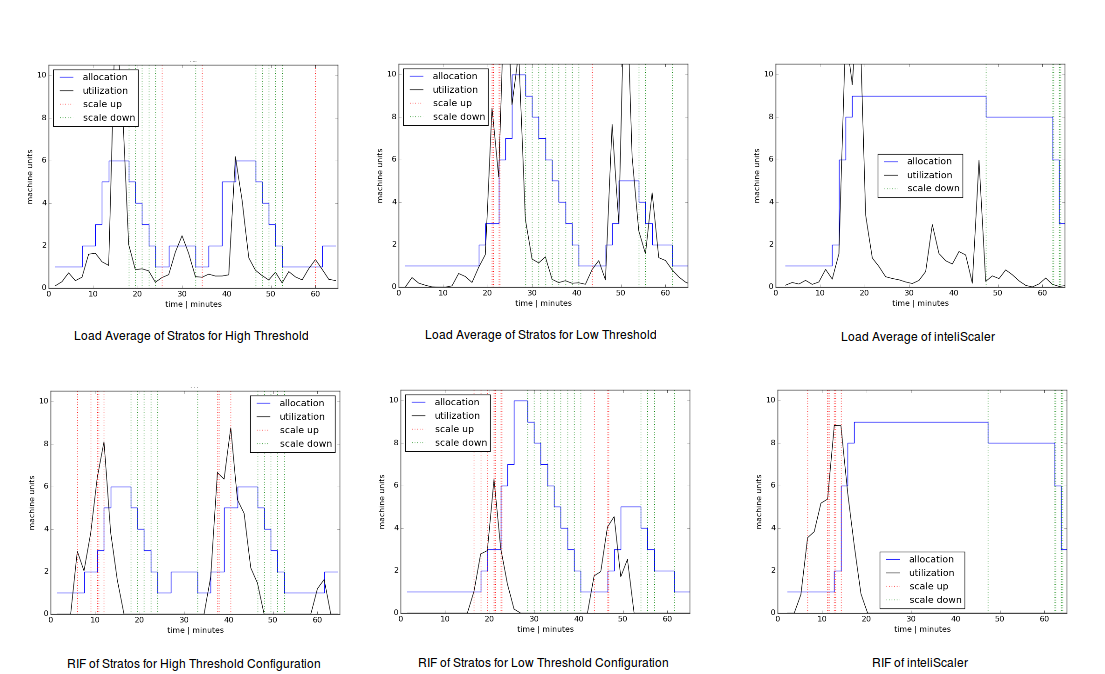
\includegraphics[width=500px]{figures/results_workload_3_4}
\caption{Performance comparison in AWS EC2 Setup for Workload I}
\label{graph:workload_3}
\end{figure}

\begin{table}[h!]
\centering
\caption{QoS summary for evaluation for Workload I on AWS EC2}
\label{table:analysis_qos_workload_3}
\begin{tabular}{|l|c|c|c|c|c|}
\hline

test case & average  response time & requests initiated & requests completed  & time out errors \\ \hline

low threshold & 6.3839 s & 254535 & 203067 & 2511\\ \hline

high threshold & 4.4954 s & 280477 & 191891  & 11863\\ \hline

inteliScaler & 5.1288 s & 286180 & 261979  & 2278\\ \hline

\end{tabular}
\end{table}

It is clear that inteliScaler outperforms both configurations of Stratos as shown in figure \ref{graph:workload_3}. InteliScaler has allocated less number of VM's to handle the same workload. In terms of QoS inteliScaler has a success ratio of 91.54\%, which is significantly higher than, the 80\% of low threshold configuration and 68\% of high threshold configuration. Number of time out errors is also significantly low where in inteliScaler it is  0.8\%, in low threshold configuration it is 0.9\%  and in high threshold configuration it is  4.2\%. 

\pagebreak

\subsubsection{Workload II}
We also tested both Stratos and inteliScaler with a fluctuating yet growing workload as described in table \ref{table:workload_5}.
\begin{table}[h!]
\centering
\caption{Workload II for AWS Setup}
\label{table:workload_5}
\begin{tabular}{|l|l|l|l|l|l|l|l|l|l|l|}
\hline
Segment & 1 & 2 & 3 & 4 & 5 & 6 & 7 & 8 & 9 & 10\\ \hline
Duration (seconds) & 90 & 90 & 90 & 90 & 90 & 90 & 90 & 90 & 90 & 90 \\ \hline
Users & 200 & 100 & 400 & 200 & 600 & 400 & 800 & 600 & 1000 & 800   \\ \hline
Transition (seconds) & 30 & 30 & 30 & 30 & 30 & 30 & 30 & 30 & 30 & 30  \\ \hline
\end{tabular}
\end{table}
\begin{figure}[h!]
\centering
\captionsetup{justification=centering,margin=1cm}
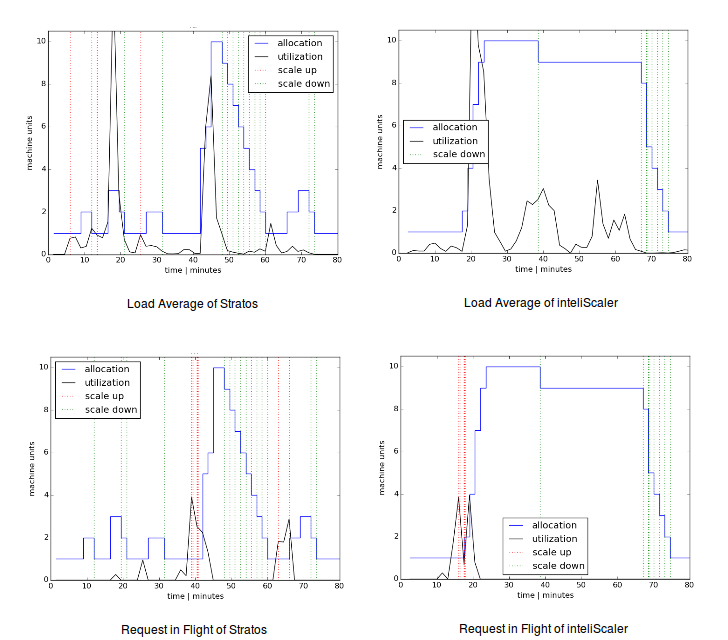
\includegraphics[width=500px]{figures/results_workload_5}
\caption{Performance comparison in AWS EC2 Setup for Workload II}
\label{graph:workload_5}
\end{figure}


\begin{table}[h!]
\centering
\caption{QoS summary for evaluation of Workload II on AWS EC2}
\label{table:analysis_qos_workload_5}
\begin{tabular}{|l|c|c|c|c|c|}
\hline

test case & average  response time & requests initiated & requests completed & time out errors \\ \hline

Stratos & 2.7150 s & 178848 & 102671 & 16257\\ \hline

inteliScaler & 1.1207 s & 214041 & 201719 & 6988\\ \hline

\end{tabular}
\end{table}

As shown in figure \ref{graph:workload_5} inteliScaler has the lowest resource allocation of 10 VMs whereas for the same workload Apache Stratos allocates 15 VMs, saving the cost for 5 VM's. Also the QoS of inteliScaler is better than Stratos as shown in table \ref{table:analysis_qos_workload_5}. inteliScaler has responded to 94.24\% of the requests generated whereas Stratos has responded to only for 57.41\% of the total requests generated. There is a significant time out and drop off error in Stratos compared to inteliScaler, which is the reason for these figures. 
